\documentclass[border=10pt]{standalone}

\usepackage{tikz}
\usepackage{tikzsymbols}
\usetikzlibrary{calc,patterns,shapes.geometric}

\def\centerarc[#1](#2)(#3:#4:#5){\draw[#1] ($(#2)+({#5*cos(#3)},{#5*sin(#3)})$) arc (#3:#4:#5);}

\begin{document}
	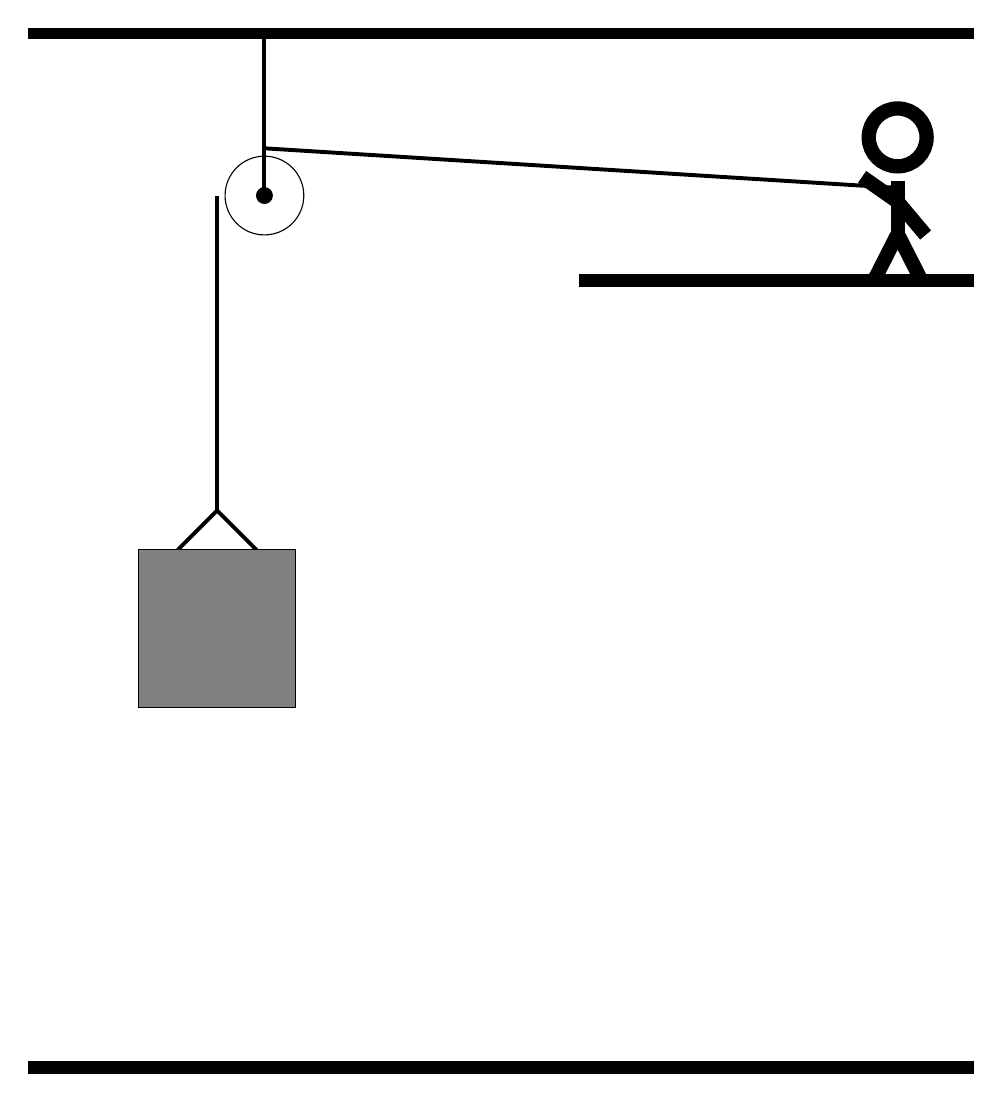
\begin{tikzpicture}
		%%%%% START %%%%%
		\draw[fill=black] (-2, 10) rectangle (10, 10.125);
		
		\draw (1, 8) circle (0.5);
		\draw[fill=black] (1, 8) circle (0.1);
		\draw[line width=0.5mm] (1, 10) -- (1, 8);
		
		\draw[line width=0.5mm](-0.1, 3.5) --  (0.4, 4.0) -- (0.9, 3.5);
		\draw[fill=black!50] (-0.6, 3.5) rectangle (1.4, 1.5);
		
		\draw[line width=0.5mm](0.4, 8) -- (0.4, 4.0);
		\centerarc[line width=0.5mm](1, 8)(90:180:0.6)
		\draw[line width=0.5mm](1, 8.6) -- (9, 8.1);
		
		\node at (9, 8) {\Strichmaxerl[10][-35][-50]};
		\draw[fill=black] (5, 7) rectangle (10, 6.85);
		
		\draw[fill=black] (-2, -3) rectangle (10, -3.15);
		%%%%% END %%%%%
	\end{tikzpicture}
\end{document}